\documentclass[10pt,a4paper]{article}
\usepackage[left=2cm,right=2cm,top=2cm,bottom=2cm]{geometry}
\usepackage[T1]{fontenc}
\usepackage{lmodern}
\usepackage[spanish,es-tabla,es-noquoting]{babel}
\usepackage[dvipsnames]{xcolor}
\usepackage[fleqn]{mathtools}
\usepackage{booktabs}
\usepackage{amsmath}
\usepackage{latexsym}
\usepackage{graphicx}
\usepackage{nccmath}
\usepackage{multicol}
\usepackage{listings}
\usepackage{tasks}
\usepackage{color}
\usepackage{float}
\usepackage{tikz}
\usetikzlibrary{arrows.meta}
\usepackage{csquotes}
\usepackage[backend=biber,style=numeric,sorting=none]{biblatex}
\addbibresource{referencias.bib}

\definecolor{colorIPN}{rgb}{0.5, 0.0,0.13}
\definecolor{colorESCOM}{rgb}{0.0, 0.5,1.0}
\graphicspath{ {imagenes/} }

\begin{document}
%#########################################################
\begin{titlepage}
	\centering
	{ \huge \bfseries \color{colorIPN}{Instituto Politécnico Nacional} \par}
	{ \Large \bfseries  \color{colorESCOM}{Escuela Superior de Cómputo} \par }
	\vspace{1cm}
	{\huge\Large \color{colorIPN}{Web Client and Backend Development Frameworks}.\par}
	\vspace{1.5cm}
	{\huge\Large  \color{colorESCOM}{Práctica: interfaz gráfica de escritorio para Carrera con JDBC y el patrón DAO}\par}
		\vspace{2cm}
	{\Large\itshape \color{colorIPN}{Profesor: Dr. José Asunción Enríquez Zárate}\par} \hfill \break
	\vspace{2cm}
	{\Large\itshape \color{colorIPN}{Alumno: Angel Frausto Robles}\par} \hfill \break
	{\Large\itshape \color{colorIPN}{Boleta: 2019630177}\par} \hfill \break
	{\Large\itshape \color{colorIPN}{id634296@gmail.com}\par} \hfill \break
	{\Large\itshape \color{colorIPN}{7CM2} \par}
	\vfill
	{\large \color{colorIPN}{\today}\par}
	\vfill
\end{titlepage}

\renewcommand\lstlistingname{Código}

\lstset{
	basicstyle=\small\sffamily,
	numbers=left,
	numberstyle=\tiny,
	frame=tb,
	tabsize=4,
	columns=fixed,
	showstringspaces=false,
	showtabs=false,
	keepspaces,
	commentstyle=\color{Violet},
	keywordstyle=\color{colorIPN} \bfseries,
	stringstyle=\color{colorESCOM},
	extendedchars=true,
	inputencoding=utf8,
	literate=
		{á}{{\'a}}1 {é}{{\'e}}1 {í}{{\'i}}1 {ó}{{\'o}}1 {ú}{{\'u}}1
		{Á}{{\'A}}1 {É}{{\'E}}1 {Í}{{\'I}}1 {Ó}{{\'O}}1 {Ú}{{\'U}}1
		{ñ}{{\~n}}1 {Ñ}{{\~N}}1 {ü}{{\"u}}1 {¿}{{?`}}1 {¡}{{!`}}1
}

\settasks{
	counter-format=(tsk[r]),
	label-width=4ex
}
\tableofcontents
\pagebreak
\listoffigures
\pagenumbering {arabic}

\pagebreak

%################################################
\section{\color{colorIPN}{Introducción}}

Esta práctica conecta una aplicación de escritorio en Java con MySQL a través de JDBC, usando el patrón DAO para que la interfaz gráfica nunca escriba SQL directamente. El recurso es \texttt{Carrera}, con cuatro operaciones: alta, baja, cambio y consulta. La clase \texttt{CarreraDAO} concentra el acceso a datos con \texttt{PreparedStatement}, y la clase \texttt{VentanaCarrera} (Swing) dispara esos métodos según el botón que se presione.

%################################################
\section{\color{colorIPN}{Desarrollo de la aplicación}}

\subsection{La tabla en la base de datos}

La base \texttt{MisCursos} corre en un contenedor de MySQL 8 (\texttt{docker-compose.yml} de esta misma carpeta), con la tabla creada desde el script de inicialización. La figura \ref{img:describe} muestra la estructura real de la tabla, obtenida con \texttt{describe Carrera;} contra el contenedor en ejecución.

\begin{figure}[H]
	\centering
	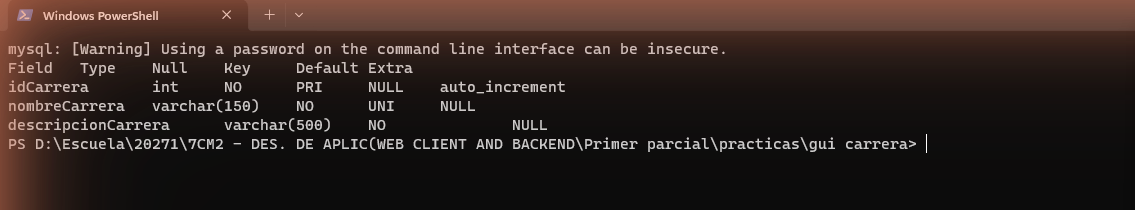
\includegraphics[width=0.85\linewidth]{00_describe_carrera.png}
	\caption{Estructura real de la tabla Carrera (\texttt{describe Carrera;})}
	\label{img:describe}
\end{figure}

\subsection{Las clases DAO y PreparedStatement}

\texttt{CarreraDAO} tiene un método privado, \texttt{obtenerConexion()}, que carga el driver de MySQL y abre la conexión JDBC. Los cinco métodos públicos (\texttt{create}, \texttt{read}, \texttt{readAll}, \texttt{update}, \texttt{delete}) llaman primero a ese método y después arman una consulta con \texttt{PreparedStatement}, nunca concatenando el SQL con los valores a mano:

\begin{lstlisting}[caption={Alta de una carrera con PreparedStatement}]
public void create(Carrera c) throws SQLException {
    obtenerConexion();
    PreparedStatement ps = conexion.prepareStatement(SQL_INSERT);
    ps.setString(1, c.getNombreCarrera());
    ps.setString(2, c.getDescripcionCarrera());
    ps.executeUpdate();
    ps.close();
    conexion.close();
}
\end{lstlisting}

El \texttt{PreparedStatement} cumple dos funciones a la vez. Evita la inyección SQL, porque los valores se mandan por separado del texto de la consulta y no se pegan directamente en la cadena. Y de paso deja el texto del SQL fijo como constante (\texttt{SQL\_INSERT}), en vez de reconstruirlo en cada llamada.

\texttt{VentanaCarrera} no importa ninguna clase de \texttt{java.sql}: solo conoce a \texttt{CarreraDAO} y a \texttt{Carrera}, y reacciona a las excepciones que el DAO declara (\texttt{SQLException}) mostrando un cuadro de diálogo. Esa es la separación que el patrón DAO impone entre la interfaz y el acceso a datos \cite{alur2003corej2ee}.

\subsection{La interfaz gráfica y el CRUD}

La ventana arranca con solo los botones \textbf{Nuevo} y \textbf{Listar} habilitados (figura \ref{img:inicial}). Al dar de alta una carrera se habilita el formulario y el botón \textbf{Guardar}; al guardar, \texttt{CarreraDAO.create()} inserta el registro real en MySQL y la tabla se refresca leyendo de vuelta con \texttt{readAll()} (figuras \ref{img:alta1} y \ref{img:alta2}).

\begin{figure}[H]
	\centering
	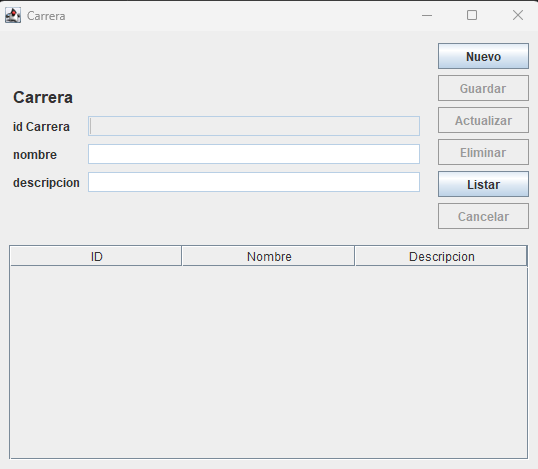
\includegraphics[width=0.95\linewidth]{01_estado_inicial.png}
	\caption{Estado inicial: solo Nuevo y Listar habilitados, tabla vacía}
	\label{img:inicial}
\end{figure}

\begin{figure}[H]
	\centering
	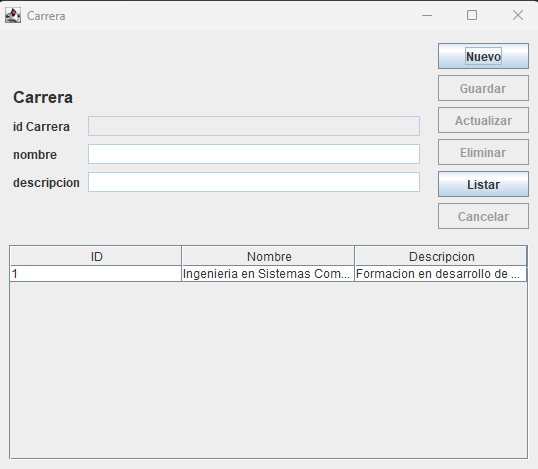
\includegraphics[width=0.95\linewidth]{02_alta_carrera1.png}
	\caption{Alta de la primera carrera, ya reflejada en la tabla tras Guardar}
	\label{img:alta1}
\end{figure}

\begin{figure}[H]
	\centering
	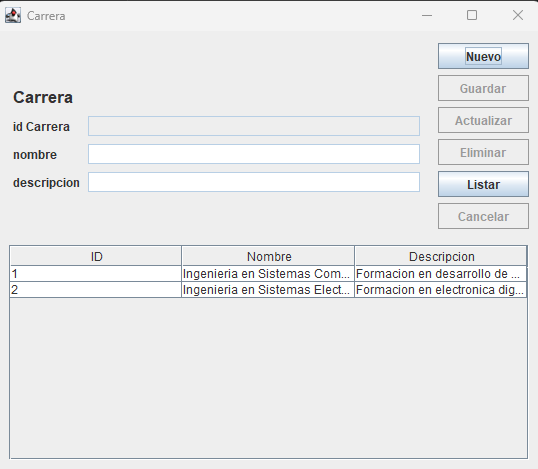
\includegraphics[width=0.95\linewidth]{03_alta_carrera2.png}
	\caption{Segunda alta, para tener dos registros y probar actualizar/eliminar}
	\label{img:alta2}
\end{figure}

Al seleccionar una fila de la tabla se habilitan \textbf{Actualizar} y \textbf{Eliminar}, y el formulario se llena con los datos de esa fila (el id queda de solo lectura). La figura \ref{img:actualizar} muestra la carrera 1 después de modificar su descripción y presionar \textbf{Actualizar}: el cambio ya viene de una consulta \texttt{UPDATE} real contra la base.

\begin{figure}[H]
	\centering
	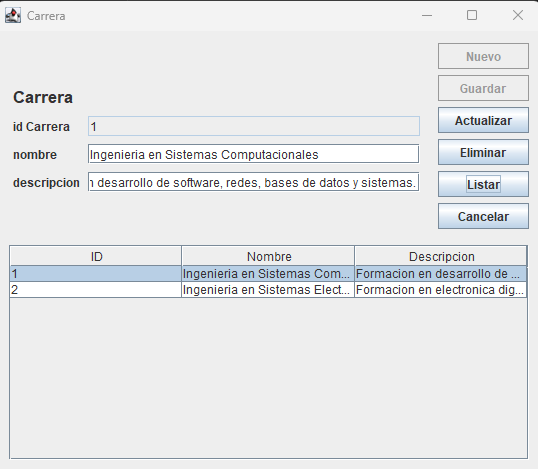
\includegraphics[width=0.95\linewidth]{04_actualizar_carrera1.png}
	\caption{Carrera 1 con la descripción actualizada vía JDBC}
	\label{img:actualizar}
\end{figure}

Eliminar pide confirmación antes de ejecutar el \texttt{DELETE} (figura \ref{img:confirmar}), y una vez confirmado la fila desaparece de la tabla porque vuelve a leerse de la base (figura \ref{img:final}).

\begin{figure}[H]
	\centering
	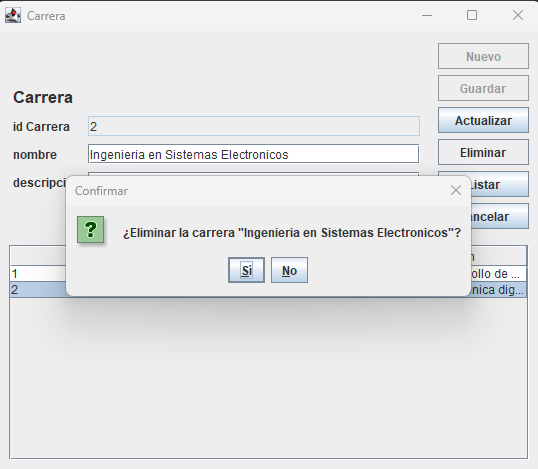
\includegraphics[width=0.95\linewidth]{05_confirmar_eliminar.png}
	\caption{Confirmación antes de eliminar la carrera 2}
	\label{img:confirmar}
\end{figure}

\begin{figure}[H]
	\centering
	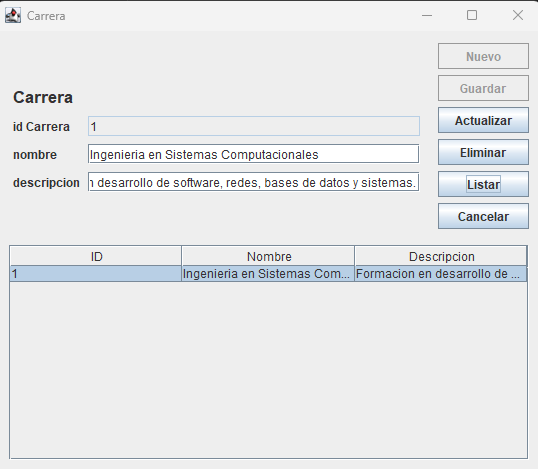
\includegraphics[width=0.95\linewidth]{06_estado_final.png}
	\caption{Estado final: solo queda la carrera 1, ya actualizada}
	\label{img:final}
\end{figure}

\subsection{Evidencia de conexión JDBC y operaciones realizadas}

Para confirmar que la interfaz gráfica en verdad llega hasta la base (y no solo actualiza una lista en memoria), la figura \ref{img:jdbc} corre \texttt{select * from Carrera;} directo contra el contenedor de MySQL, después de terminar la secuencia de alta, actualización y baja hecha desde la ventana. El único registro que queda y su descripción coinciden exactamente con lo que muestra la figura \ref{img:final}.

\begin{figure}[H]
	\centering
	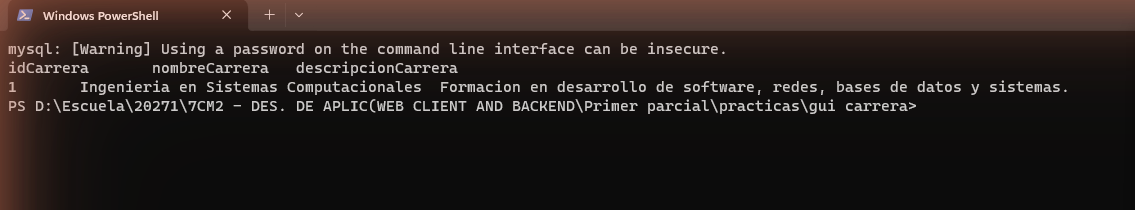
\includegraphics[width=0.85\linewidth]{07_evidencia_jdbc.png}
	\caption{Contenido real de la tabla tras las operaciones hechas desde la GUI}
	\label{img:jdbc}
\end{figure}

%################################################
\section{\color{colorIPN}{Conclusiones}}

Todas las excepciones que puede lanzar \texttt{CarreraDAO} caen bajo \texttt{SQLException}: falla de conexión, violación de la restricción \texttt{UNIQUE} en \texttt{nombreCarrera} al repetir un nombre, o un id que ya no existe al intentar actualizar o eliminar. \texttt{ClassNotFoundException} solo aparece si el conector de MySQL no está en el classpath, y por eso \texttt{obtenerConexion()} la atrapa y la convierte en \texttt{SQLException} para que el resto del DAO declare un único tipo de error.

El error más común al conectar por JDBC no es de código sino de configuración: la URL, el usuario o la contraseña no coinciden con el contenedor que en verdad está corriendo. Con el contenedor apagado o el puerto equivocado, la excepción llega igual hasta la GUI, pero como un mensaje de conexión rechazada en vez de un problema de SQL. Repetir un nombre de carrera es el segundo error típico, y es justo el que la restricción \texttt{UNIQUE} de la tabla convierte en una excepción controlada en vez de en un registro duplicado silencioso.

Separar \texttt{CarreraDAO} de \texttt{VentanaCarrera} tuvo un efecto concreto en esta práctica: cambiar la descripción de una carrera, agregar una fila o quitarla nunca tocó una línea de la ventana, porque toda esa lógica vive en el DAO. Esa es la relación entre el patrón DAO y la separación de responsabilidades que pedía el objetivo de la práctica, y coincide con lo que documenta el catálogo Core J2EE Patterns sobre este patrón \cite{alur2003corej2ee}.

%################################################
\section{\color{colorIPN}{Referencias Bibliográficas}}
\nocite{*}
\color{colorESCOM}{
	\printbibliography[heading=none]
}

\end{document}
